\chapter{Conclusions}
Revisiting figure \ref{fig:coilarea}, but multiplying
the coil areas with the solenoid field strength ($80$ mT)
we get figure \ref{fig:coilarea-weber}. This gives us an approximate
lower limit of induced flux that gives a reasonable signal 
to noise ratio. As can be seen, an induced flux of less than around
4 mWb gives a very noisy signal. Depending on magnet strength,
coil areas should be sufficiently large as to 
ensure this amount of minimum flux.

\begin{figure}[!h]
    \centering
    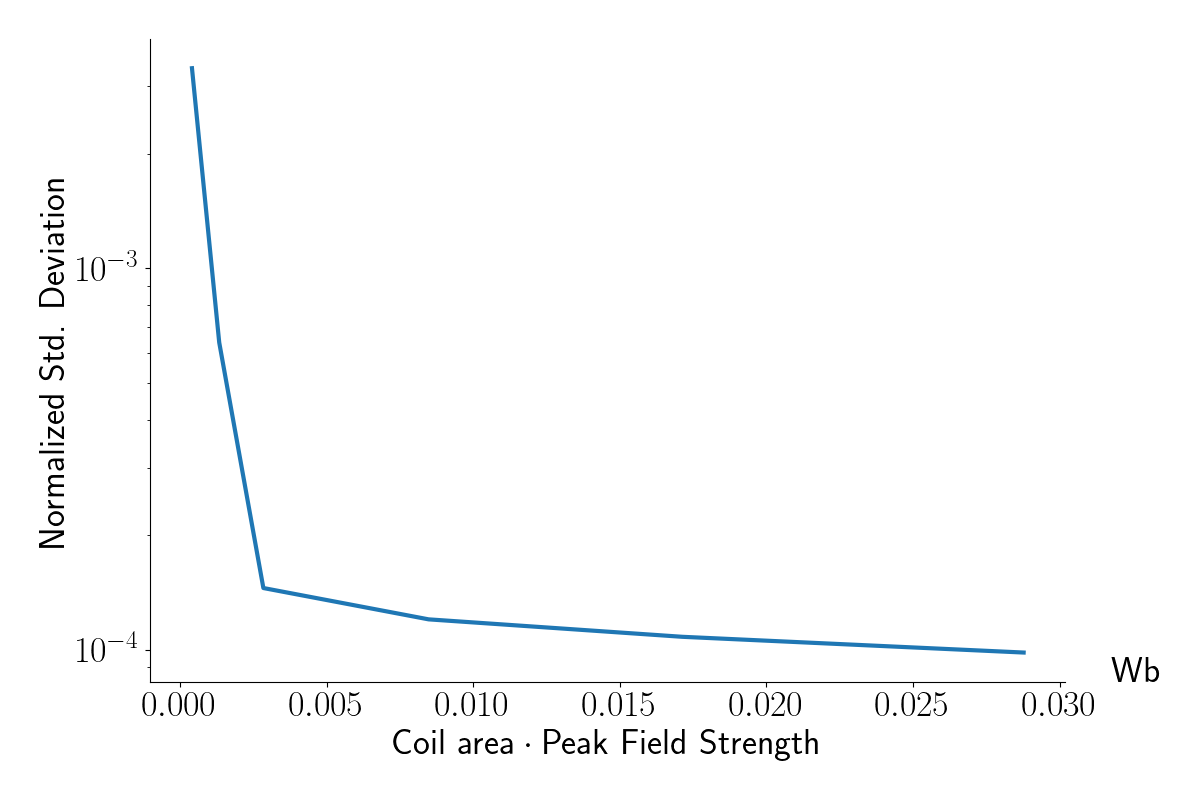
\includegraphics[width=0.8\linewidth]{figs/areatofield}
    \caption{Normalized measurement std. deviation as a function of
        induced flux.}
    \label{fig:coilarea-weber}
\end{figure}

The current sensitivity to yaw angle misalignment was estimated
to be about 4.29 mrad in section \ref{sec:peak-shift-measurements}.
The peak shifts used to characterize this misalignment is a
result of the higher order harmonics as stated in section
\ref{subsubsection:solenoid-harmonics}. To increase this
sensitivity, future coils need to be designed to more
sensitive to these harmonics. Increasing coil area is
of course one possibility, but the shape of the coil can
also be optimized. To capture the harmonics in $\varphi$,
coils spanning a smaller sector angle could be used. Such
coils are already in the pipeline to be tested at the time
of writing.

The angle estimation from the peak shifts turned out to be 
a harder problem than expected. As the arguments of the maximums of the
$B_z$ field is not easily modeled with regards to the offset, finding
a consistent model is a challenge. Some hope remains however. In figure
\ref{fig:sim-mag-fieldmap-argmax} one can see that the argmax is more affine
for densely wound solenoids with a homogenous field profile inside the aperture.
Through extensive data collection using even more simulations it might be
possible to make a working linear model. Moreover, since the error is 
decreasing with the pitch/yaw angle, this model is still viable 
for use in alignment. Since the alignment process is done iteratively,
measuring and then aligning as needed, the error will decrease with 
each iteration, trending towards zero as smaller and smaller alignments
are needed.

Another possibility is to add coils or Hall effect sensors that measure
the transversal $B_x$ and $B_y$ components. If the results of section 
\ref{sec:dipole-simulations} hold for real and not only simulated magnets,
this could be a very robust way of measuring the tilt-swing angle of the
solenoid. Although the transversal dipole moments are not as strong as
the $B_z$ field, the integral operation of the translating measurements
removes a lot of the zero-mean gaussian noise. This coupled with the fact the dipole
integral is invariant to potential offset alignment errors makes for
a promising measurement methodology. From equations 
\ref{eq:Bzlineint} and \ref{eq:tanhalf}, the 
yaw-pitch angle could then be estimated using

\begin{align}
    I_{Bz} = \int B_z dz, \; 
    I_{Bx} &= \int B_y dz, \; 
    I_{By} = \int B_x dz \\
    \theta_x &\approx 2\arctan(\frac{I_{By}}{I_{Bz}})\\
    \theta_y &\approx 2\arctan(\frac{I_{Bx}}{I_{Bz}})
\end{align}

where $\theta_x$ is the pitch angle around the x axis,
$\theta_y$ is the yaw angle around the y axis, and the 
integrals are taken over the whole measurements, where
the measurements begin and end far away from the magnet
in the zero field region.

One particularly interesting result with regards to the fitting
of the BFF series is that only the outermost coils measurements
were needed for a good fit. The innermost coils did not add any
more information. This fits well with the theory on partial
differential equations. A PDE may be completely determined
by its values at its boundaries. This also adds robustness to the system,
since the weaker field in the middle of the aperture can be estimated
using measurements of the stronger field closer to the solenoid edge,
from the more sensitive outer coils.